105. а) Катет $LM$ лежит напротив угла в $30^\circ,$ значит $LK=2LM=17.$ Для точной оценки $LN=KM$ придётся немного забежать вперёд и применить теорему Пифагора: $KM^2+8,5^2=17^2,\ PR^2=216,75.$ Это значит, что длина $LN$ лежит между 14 и 15.\\
б)\begin{figure}[ht!]
\center{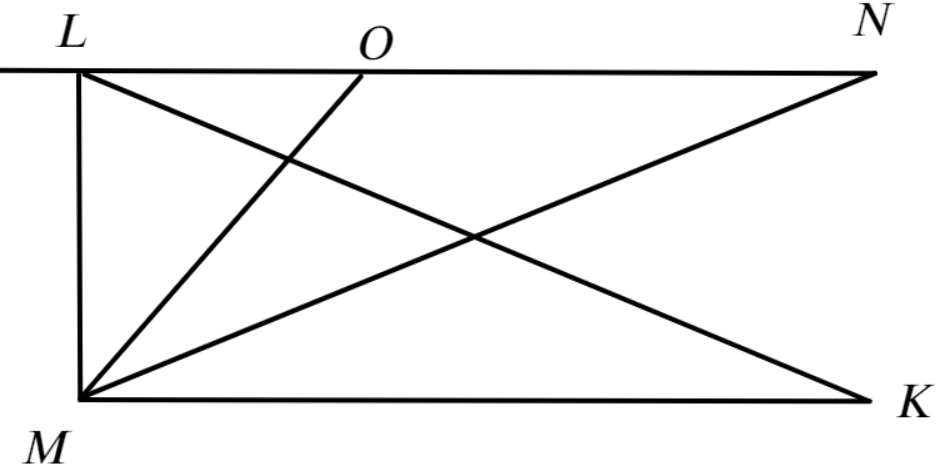
\includegraphics[scale=0.35]{g105.png}}
\end{figure}\\
Треугольники $LMN$ и $LMK$ равны по двум катетам ($LM$ общий, $LN=KM),$ значит $\angle LMN=\angle MLK=60^\circ.$ Тогда $\angle OMN=60^\circ:2=30^\circ,\ \angle MOL=90^\circ-30^\circ=60^\circ,\ \angle MON=180^\circ-60^\circ=120^\circ,\ \angle ONM=180^\circ-120^\circ-30^\circ=30^\circ.$ Точка $N$ также может лежать с другой стороны от точки $L,$ что ничего не меняет, так как получившийся треугольник будет симметричен исходному относительно $LM.$\\
